%important---今年新要求：最多不超过5页
\section{Our Big Family}
\ 

%经过指导老师的引导，相关培训和选拔后，成立了ASC竞赛队伍。作为学校的第二年ASC竞赛队伍，我们经过了较长时间的筹备，并受到了校内外许多人的帮助，我们感谢他们的技术支持和宝贵建议，使我们能够顺利地参加这次比赛。接下来详述团队的组建和团队情况。
Under the guidance of our advisors, and after relevant training and selection processes, the ASC competition team was formed. 
As the second ASC competition team of school, we underwent a lengthy preparation period and received assistance from many people both inside and outside the school, including members of the previous ASC team. 
We are grateful for their technical support and valuable suggestions, which enabled us to participate in this competition successfully. 
The following sections detail the team composition and current status.


% \textcolor{red}{to do----after 0207 }
\subsection{Setup of the team}
\ 

\begin{figure}[!htbp]
    \centering
    \subfloat{
        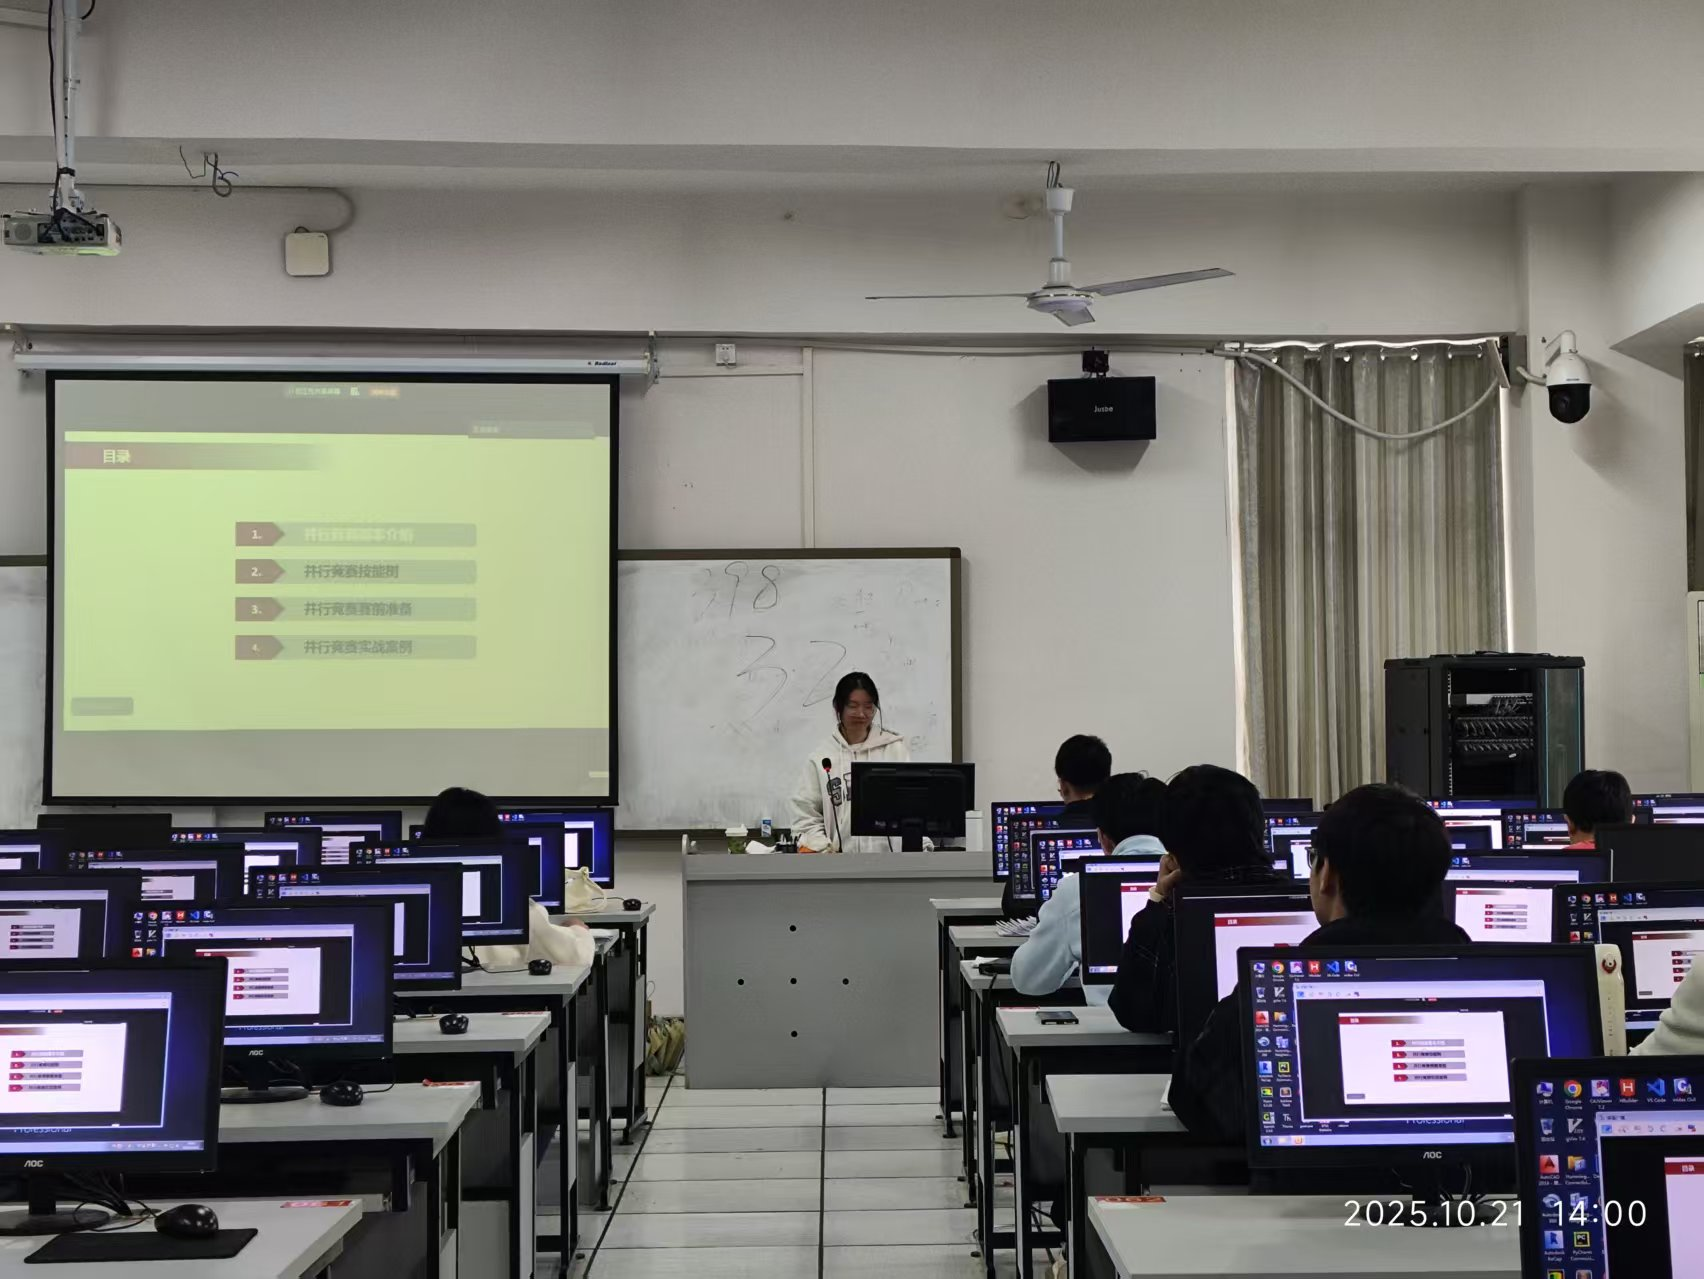
\includegraphics[width=0.48\linewidth]{figures/train0.jpg}
    } \hfill
    \subfloat{
        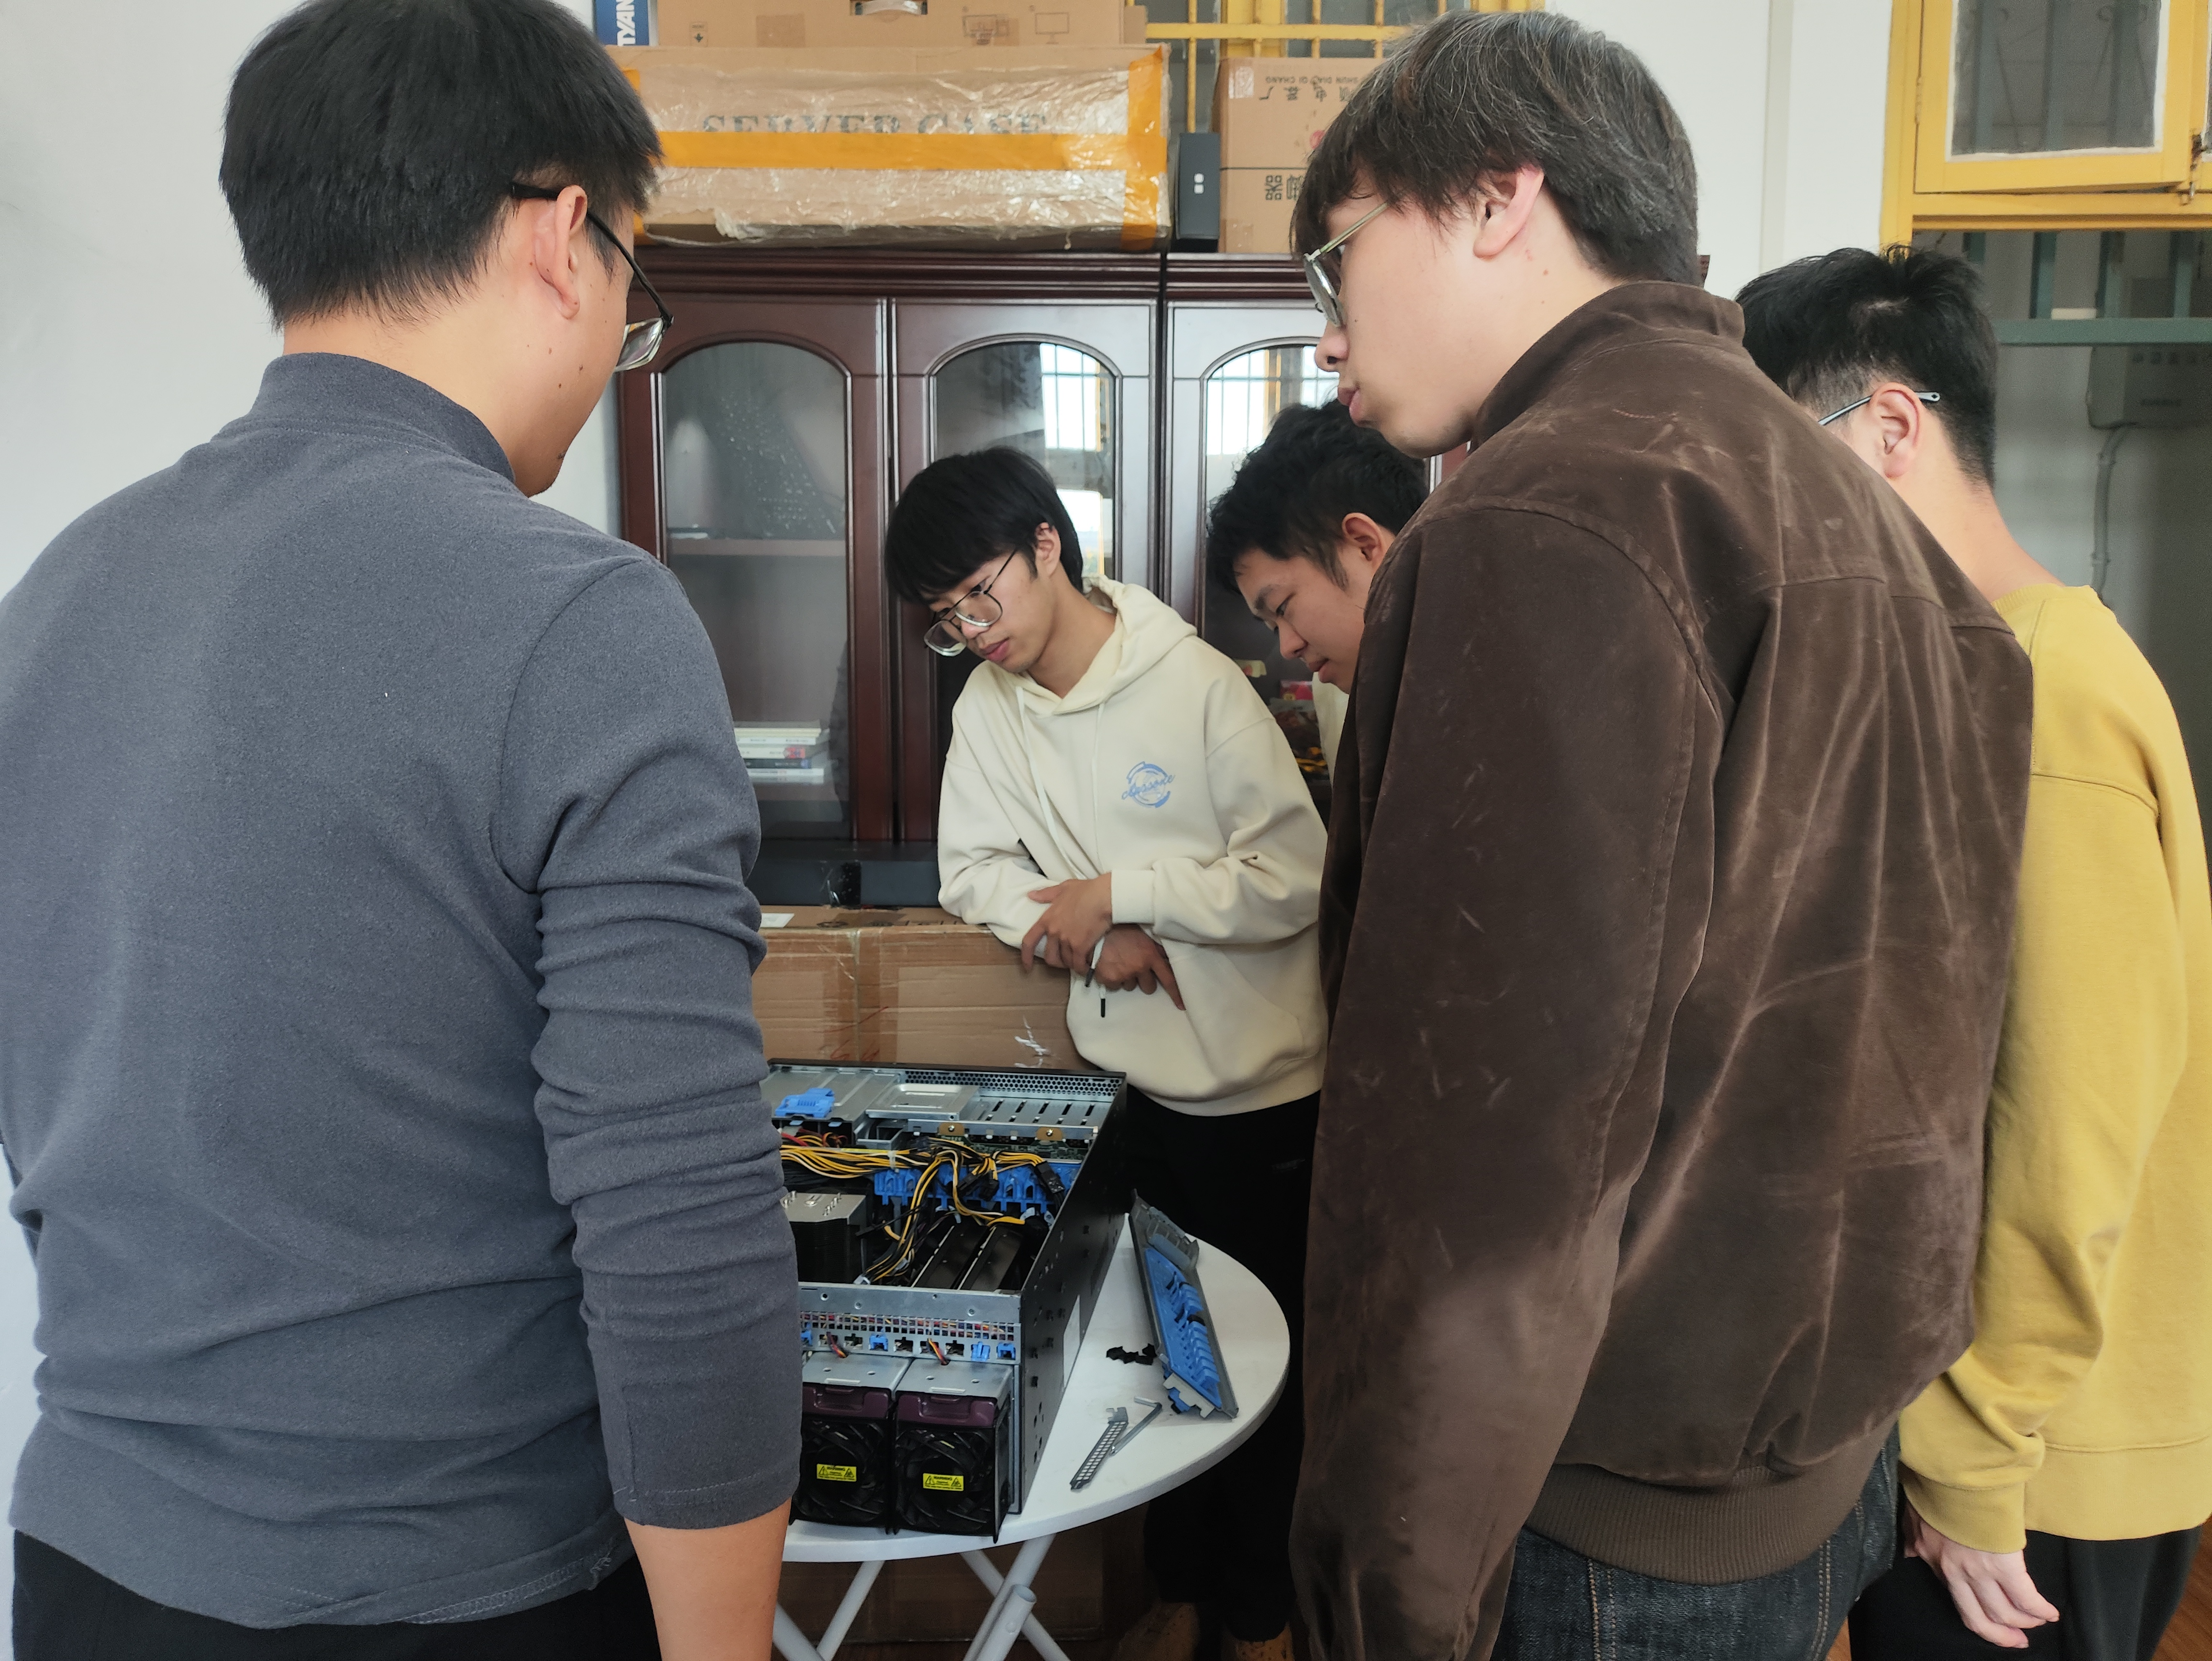
\includegraphics[width=0.48\linewidth]{figures/train1.jpg}
    } \\
    \subfloat{
        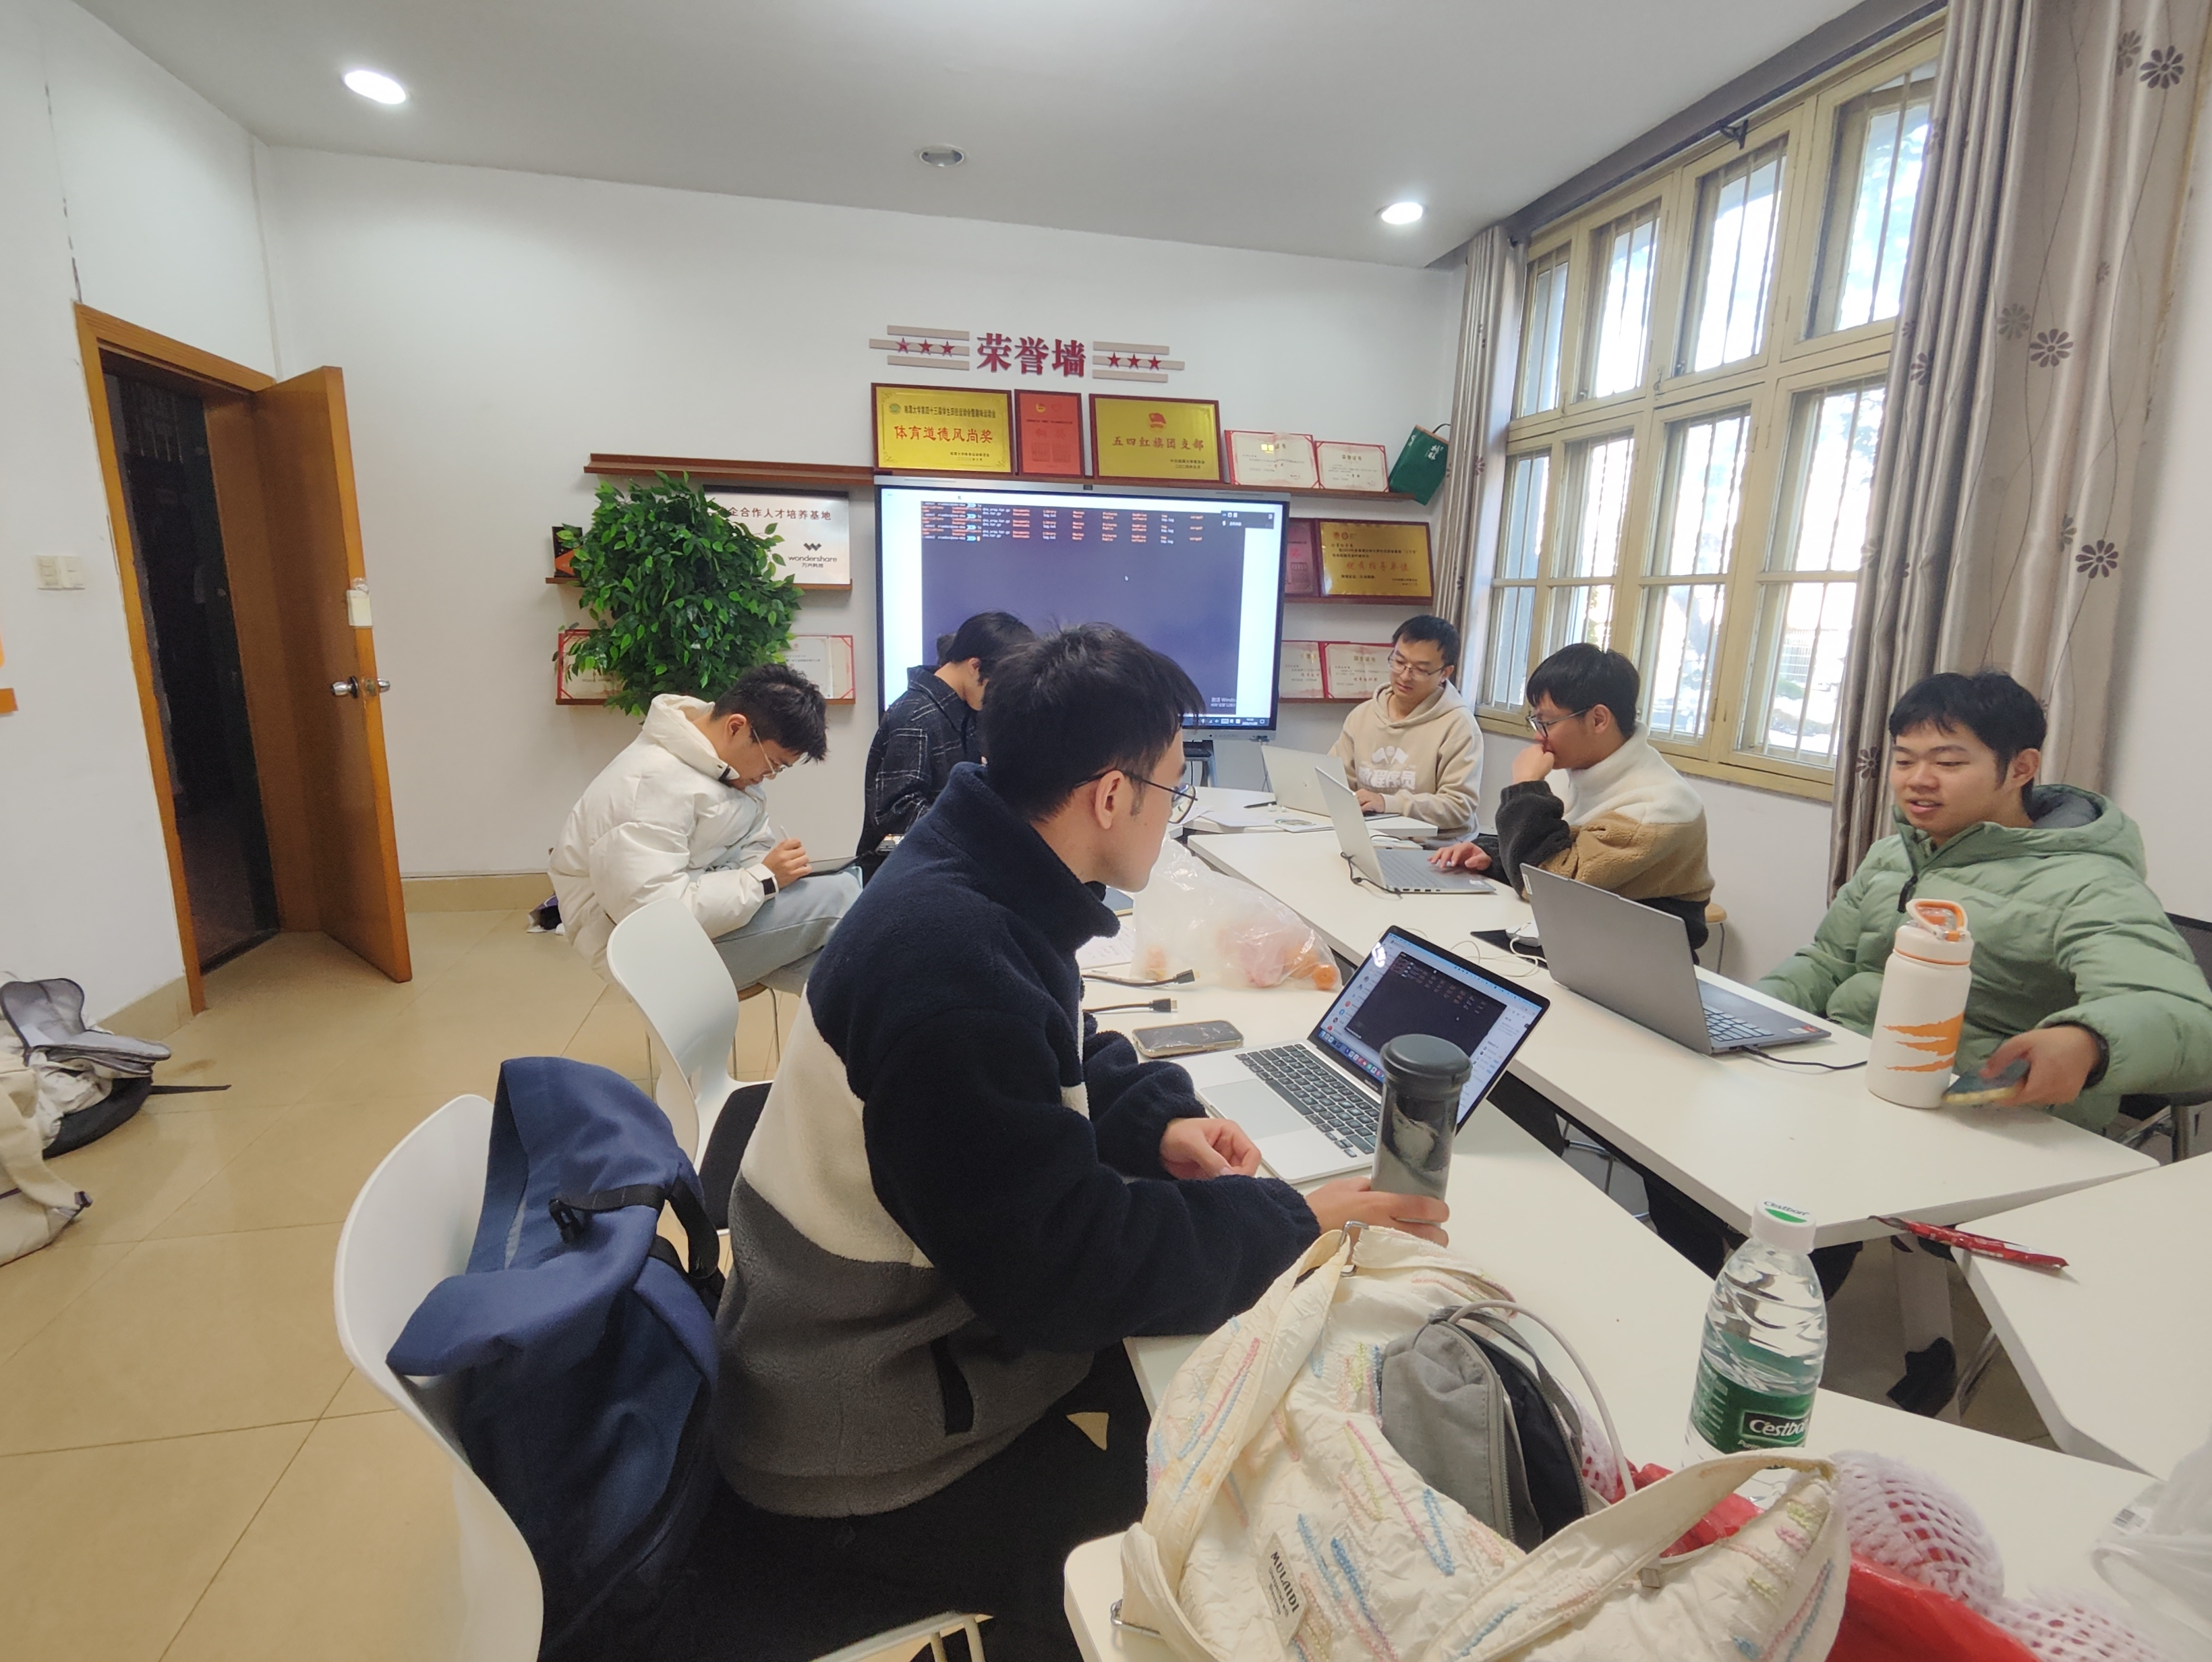
\includegraphics[width=0.48\linewidth]{figures/train2.jpg}
    } \hfill
    \subfloat{
        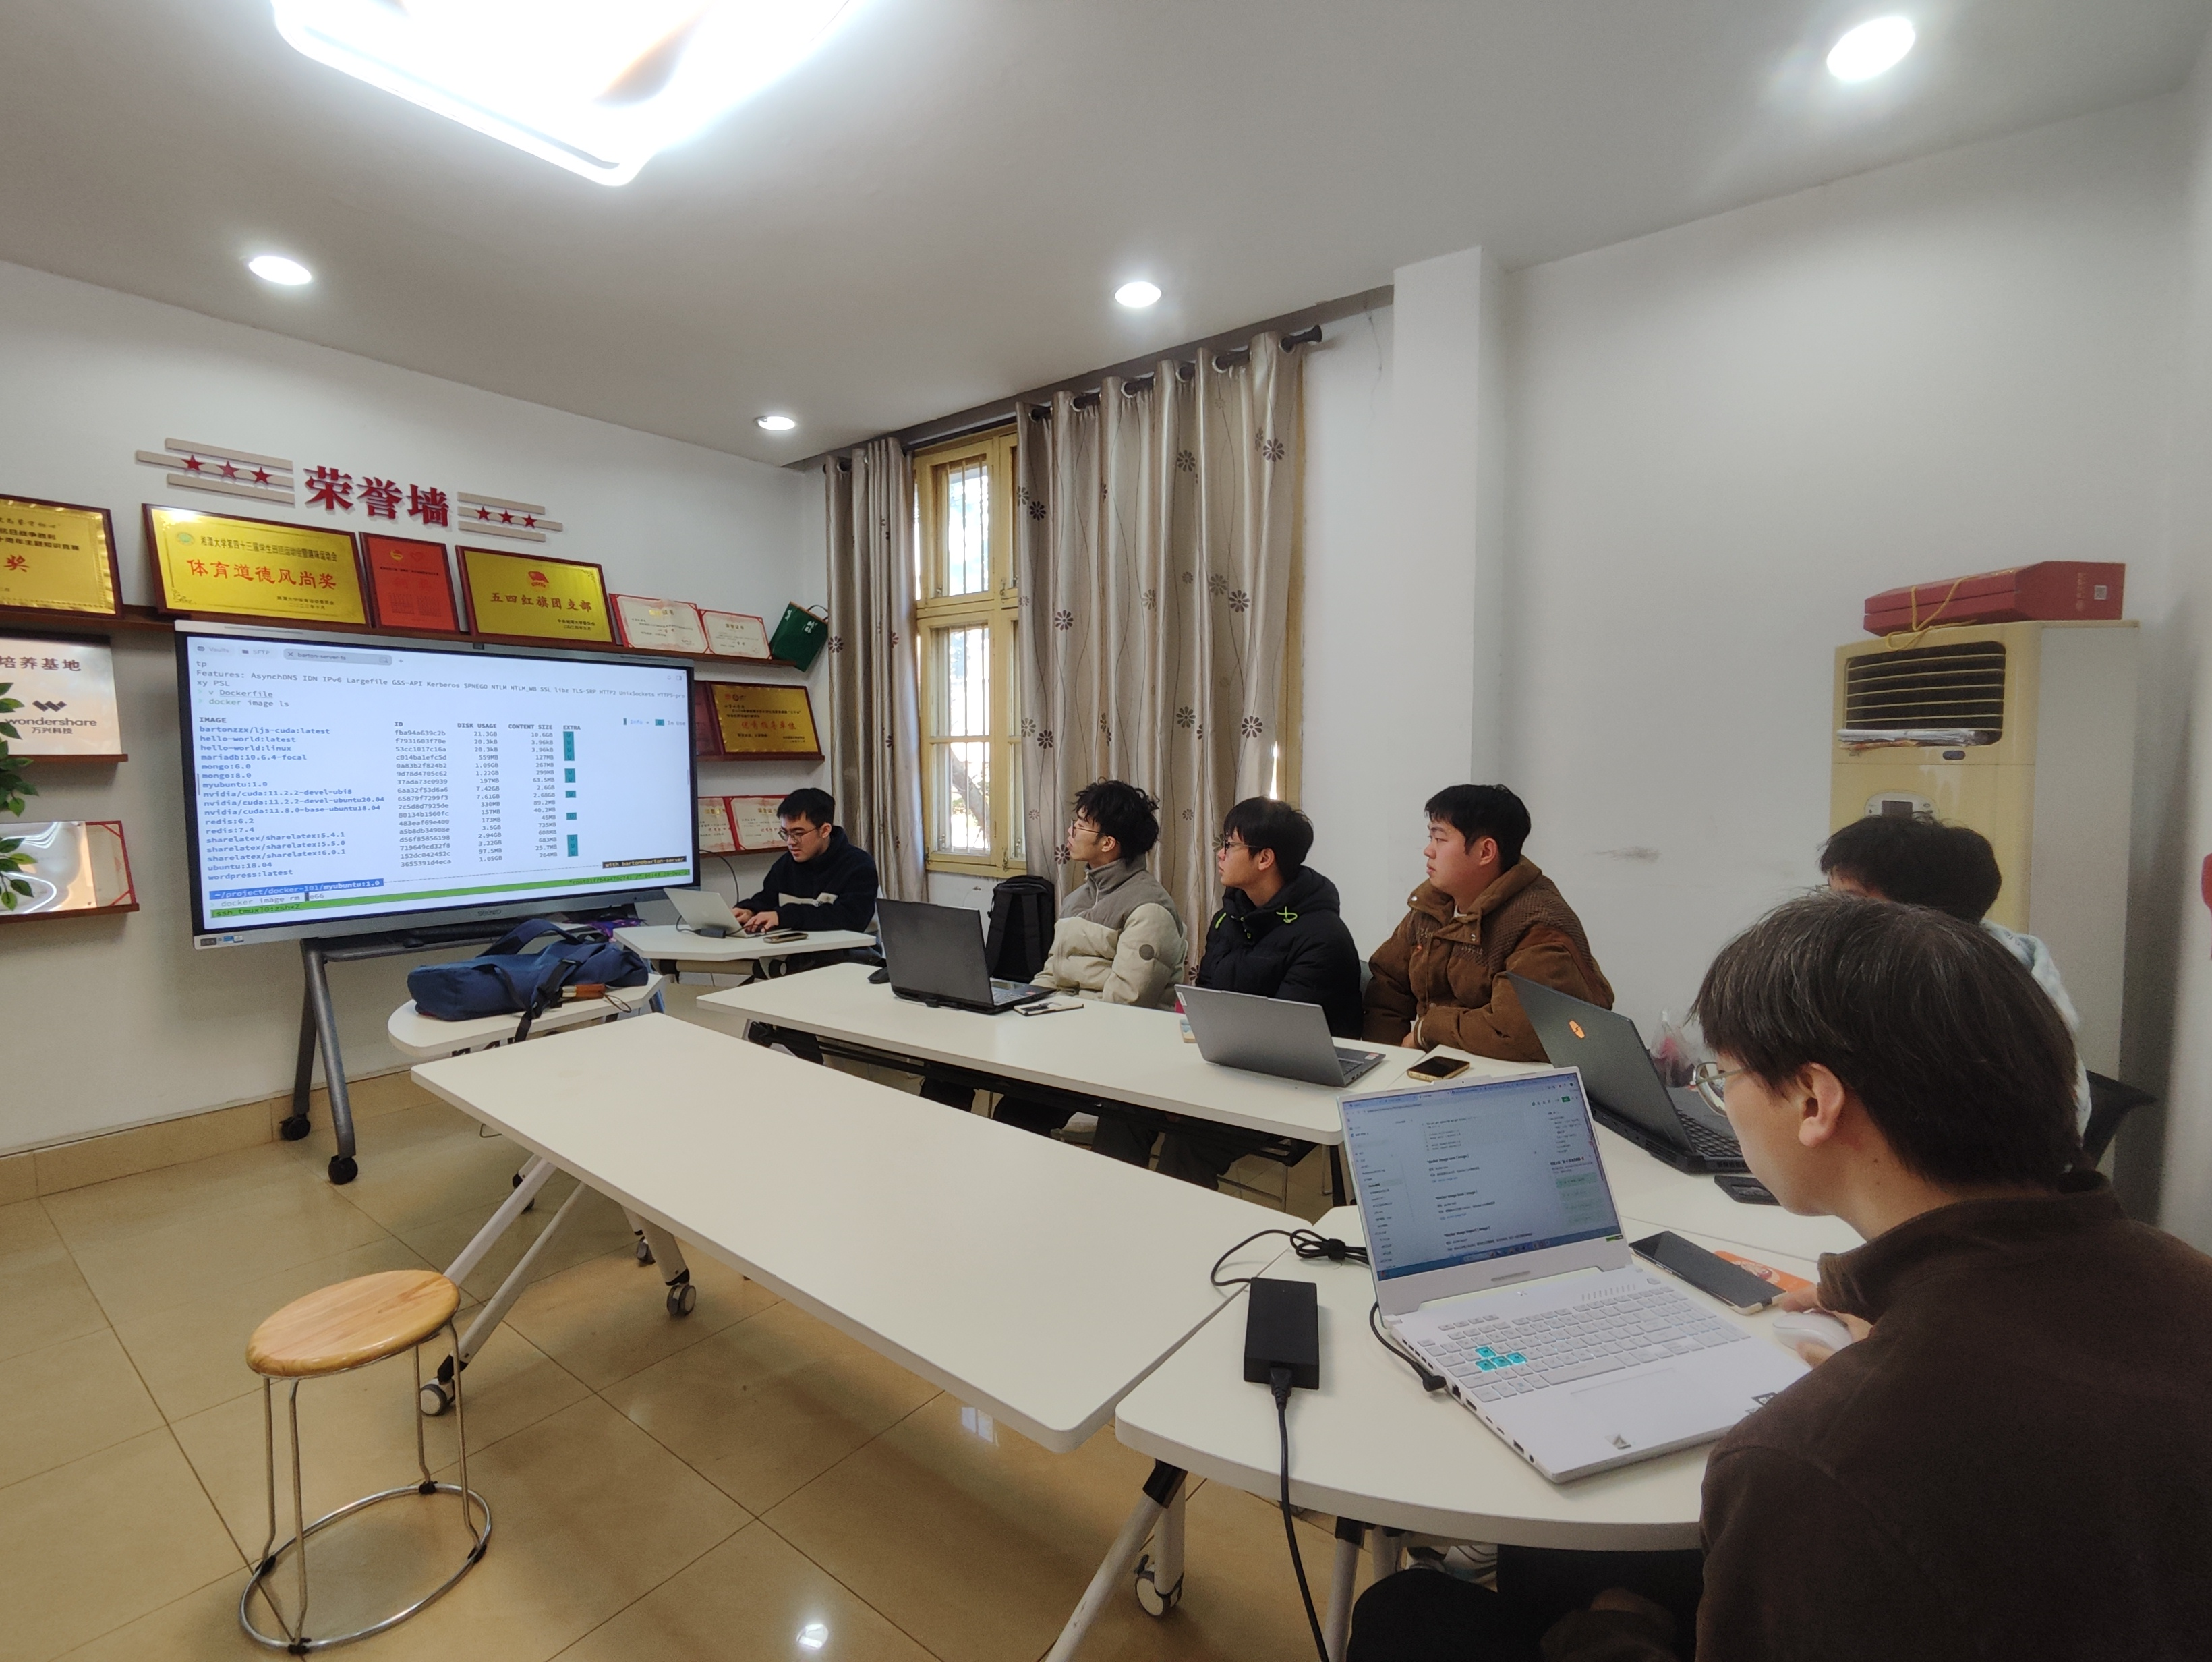
\includegraphics[width=0.48\linewidth]{figures/train3.jpg}
    } 
    \caption{Training Time}
    \label{fig:team train}
\end{figure}
% 这个比赛是由主讲并行程序设计和计算机组成原理的林培英老师发起的。林培英老师博士毕业于湖南大学，从事高性能计算研究。2024年9月开始，林老师通过课程和讲座在学校进行ASC比赛相关宣传，并制定了选拔题目。这次的比赛，从2025年9月开始，设立了新的选拔题目，然后组成了我们现在的参赛队伍。自团队成立后，林老师组织了基础知识、并行知识、优化知识等的专题培训，并多次邀请校内外前ASC参赛队员对我们进行相关经验的指导。
This competition was initiated by tutor, Peiying Lin, who teaches \textit{Parallel Programming} and \textit{Computer Organization Principles}. 
Peiying achived Ph.D. from Hunan University and is engaged in high-performance computing research. 
Starting in September 2024, Lin promoted the ASC competition through courses and lectures at the university and developed the selection criteria. 
For this year's competition, starting in September 2025, new selection criteria were established, and our current team was formed. 
Since the team's formation, Lin has organized specialized training sessions on fundamental knowledge, parallel computing, and optimization techniques, and has repeatedly invited former ASC competitors from both within and outside the university to provide guidance and share their experiences as shown in Figure \ref{fig:team train}.
% Please add the following required packages to your document preamble:
% \usepackage{subfig}



\subsection{Introduction of members}
\ 

Our participating team consists of five official members and several reserve members. 
The instructor is Peiying Lin. 
The participating students include undergraduate students majoring in Computer Science and Technology and Cyber Security. 
They are Huayu Shen, Yangkun Pei, Long Jiang, Tao Li (majoring in Computer Science and Technology, junior year) and Muyuan Chen (majoring in Cyber Security, sophomore year). 
And, the photo of our team is shown in Figure \ref{}. 
The following is an introduction of each team member.

% Please add the following required packages to your document preamble:
% \usepackage{subfig}
\begin{figure}[!htb]
    \centering
    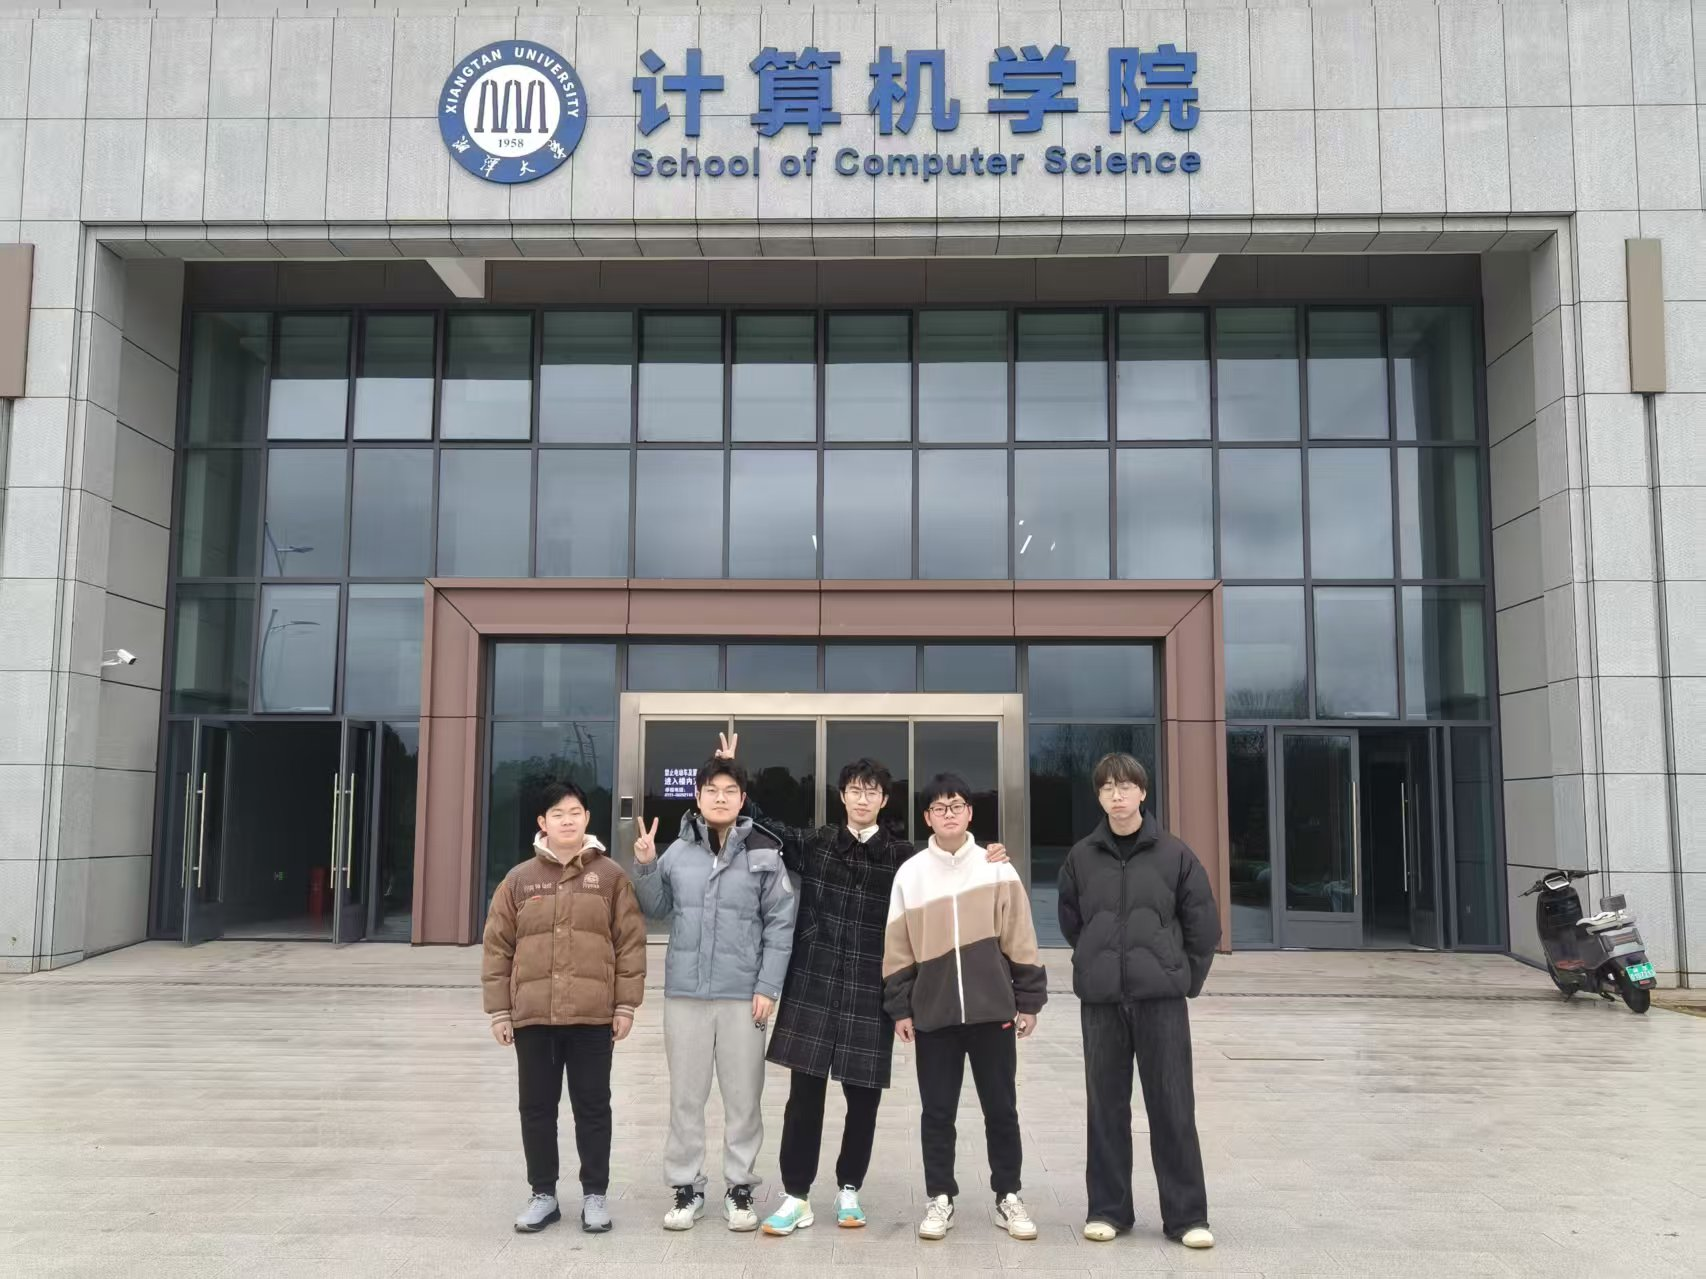
\includegraphics[width=0.7\linewidth]{figures/teammembers.jpg}
    \caption{Team Members}
    \label{fig:teams}
\end{figure}


\begin{wrapfigure}[11]{l}{0.3\textwidth} % l = 左对齐, 0.3\textwidth = 图片宽度
  \centering
  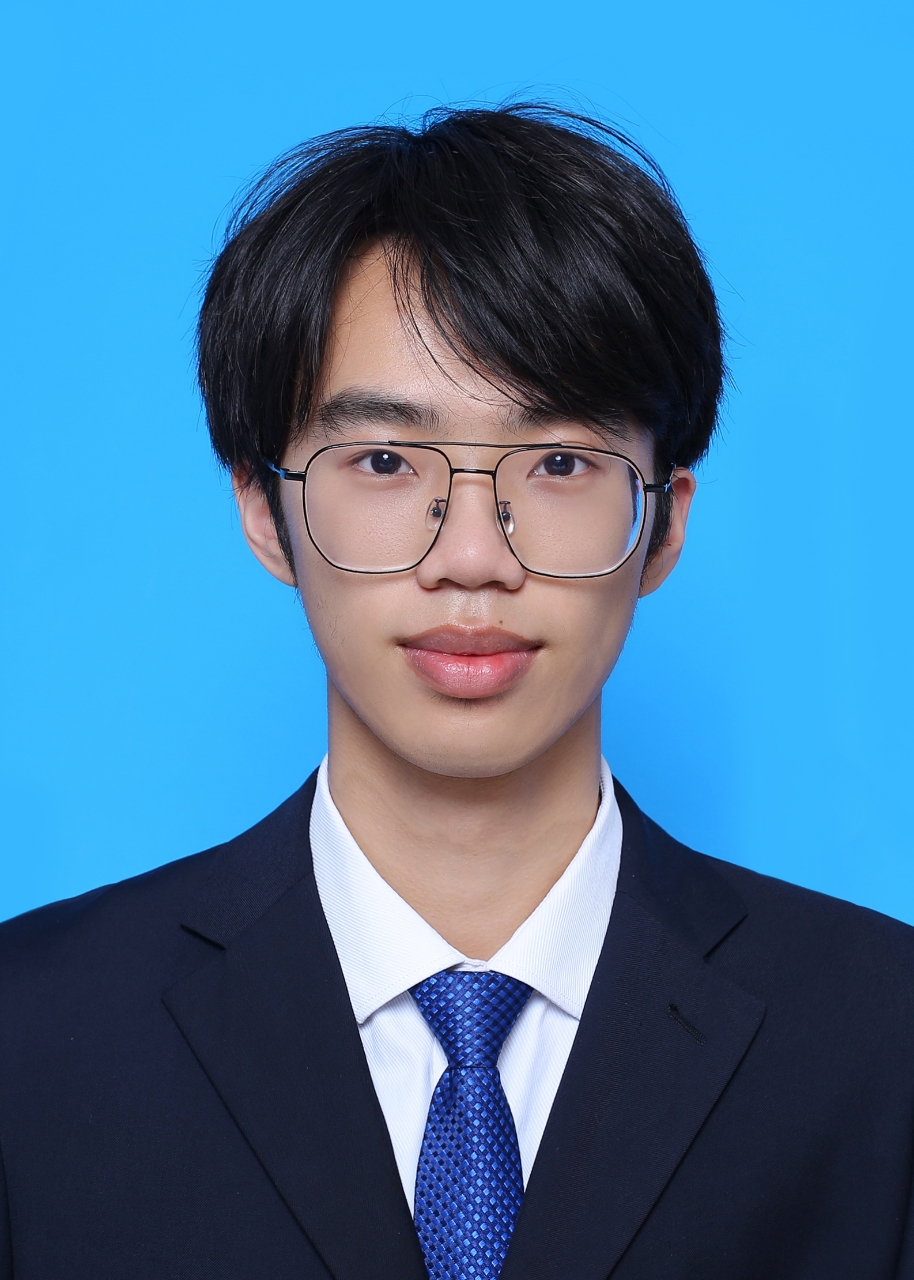
\includegraphics[height=4cm, width=3cm]{figures/teamMeambers/huayu.jpg} 
  \label{fig:huayu}
\end{wrapfigure}
\textbf{Huayu Shen}, the team leader. 
He possesses outstanding abilities to handle difficulties, solid knowledge in computer science, and a courageous spirit of exploration. 
He is proficient in the Linux system and Git version control tools, and also skilled in MPI and OpenMP multi-threading programming. 
He once participated in the development of an online learning platform as well as an intelligent course scheduling system based on genetic algorithms and multimodal optimization.
In this ASC competition, he not only managed the overall progress but also participated in the optimization of HPL tests and the performance optimization of AMSS-NCKU. 
% \vspace{1em} % 间距

\begin{wrapfigure}[10]{l}{0.3\textwidth} % l = 左对齐, 0.3\textwidth = 图片宽度
  \centering
  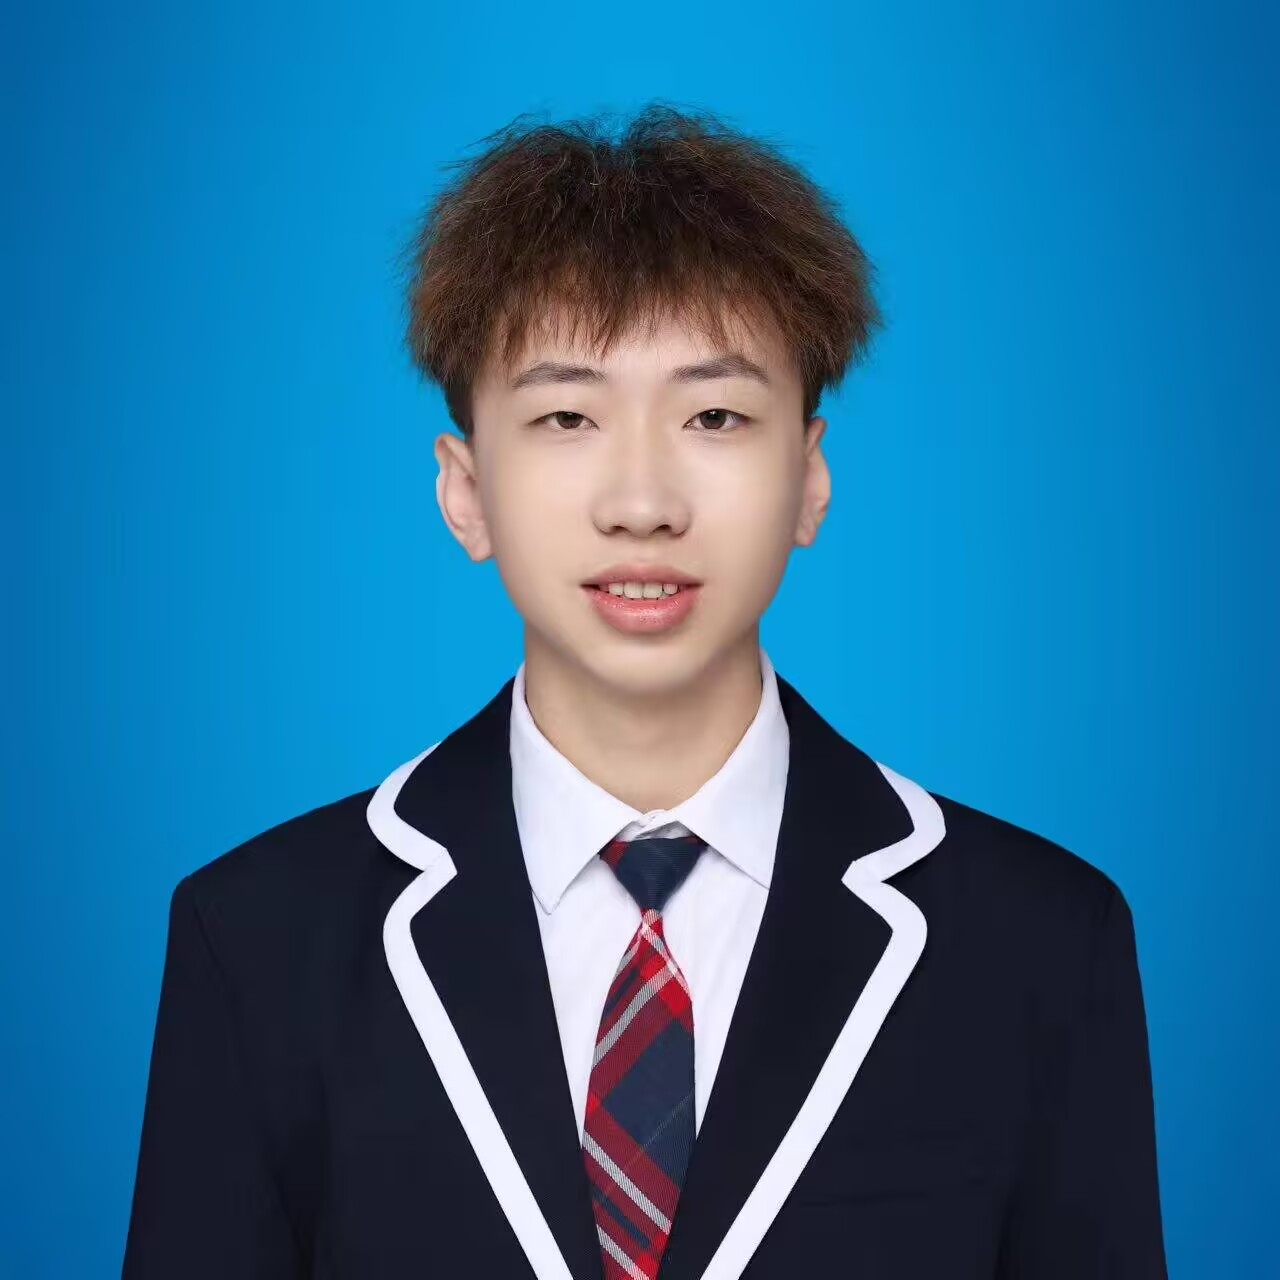
\includegraphics[height=4cm, width=3cm]{figures/teamMeambers/yangkun.jpg} 
  \label{fig:yangkun}
\end{wrapfigure}
\textbf{Yangkun Pei} is good at C/C++, Python and Shell scripting for cross-platform development, familiar with MPI, OpenMP and CUDA GPU acceleration technologies.
He possesses the ability to design and optimize multi-level parallelization algorithms. 
He is also familiar with the Linux development environment, CMake build toolchain and advanced optimization options of GCC/Intel compilers. 
In this competition, he is responsible for the deployment and operation of AMSS-NCKU and the design and implementation of its optimization plan. Additionally, he also completed the performance optimization analysis of HPCG on the CPU.
% \vspace{1em} % 间距


\begin{wrapfigure}[12]{l}{0.3\textwidth} % l = 左对齐, 0.3\textwidth = 图片宽度
  \centering
  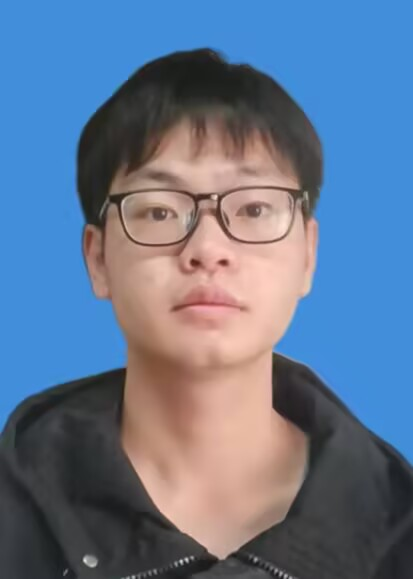
\includegraphics[height=4cm, width=3cm]{figures/teamMeambers/jianglong.jpg} 
  \label{fig:jianglong}
\end{wrapfigure}

\textbf{Long Jiang}  is skilled in mainstream programming languages, and has strong abilities in algorithm design and analysis. 
He has a deep understanding of MPI and OpenMP parallel programming models, and has a preliminary understanding of the CUDA C programming model. 
He is familiar with the Linux operating system and is proficient in using various Linux commands and uses WSL2 as his daily development platform.
He is also familiar with machine learning algorithm. 
In this competition, he takes charge of the UnifoLM-WMA-0 optimization, employing various optimization methods to achieve acceleration, such as I/O optimization, cache optimization, and operator optimization, etc. 
In addition, he was also responsible for the CPU test optimization of HPCG.


\begin{wrapfigure}[9]{l}{0.3\textwidth} % l = 左对齐, 0.3\textwidth = 图片宽度
  \centering
  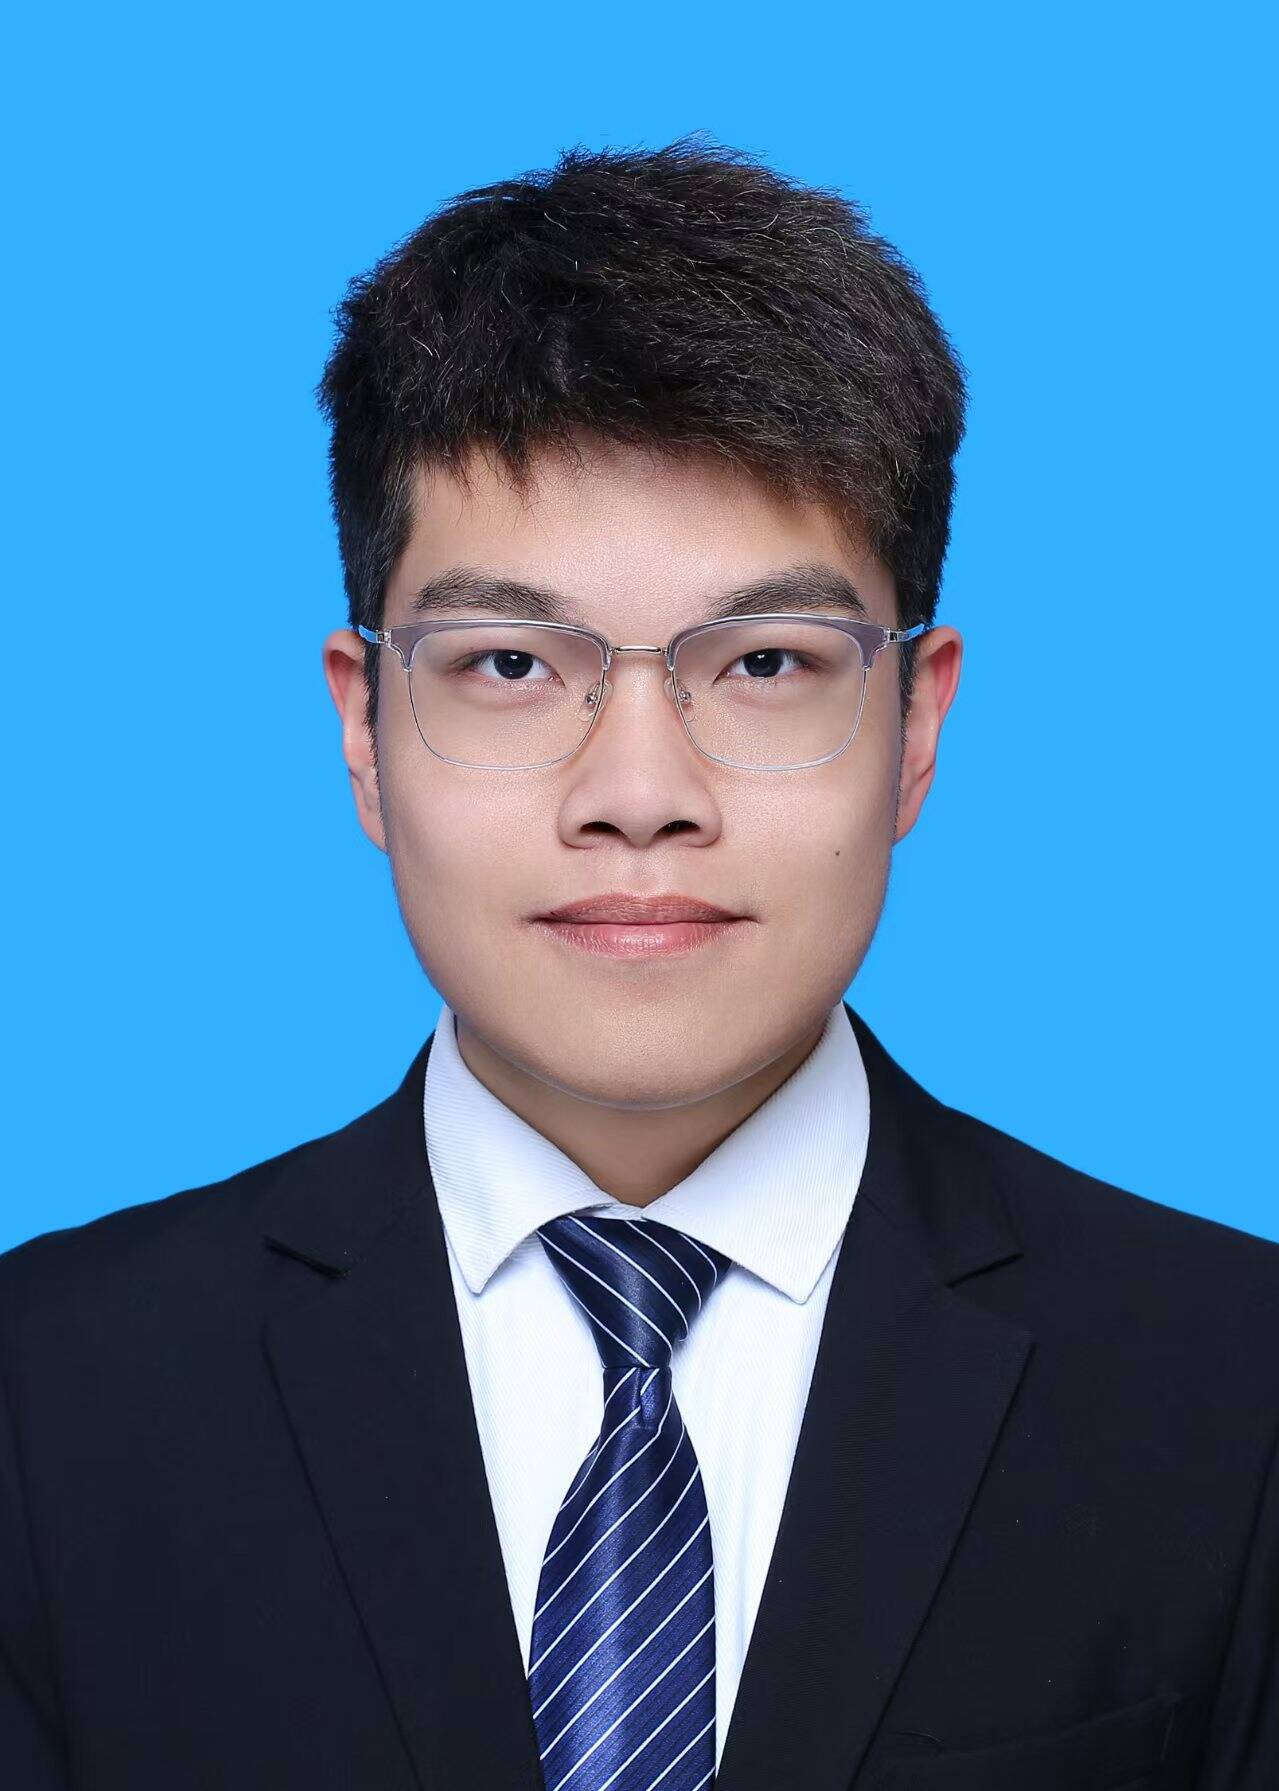
\includegraphics[height=4cm, width=3cm]{figures/teamMeambers/muyuan.jpg} 
  \label{fig:muyuan}
\end{wrapfigure}
\textbf{Muyuan Chen} has a passion for computers and possesses strong learning abilities. 
He is proficient in using Linux and Git, and is well-versed in C/C++ and Java programming languages. 
He has a strong ability in algorithm design and implementation, and can quickly adapt to different programming environments. 
He is familiar with technologies such as model inference security and security protection. 
In this competition, he mainly took charge of the HPCG GPU optimization part and the analysis and design of the UnifoLM-WMA-0 optimization.


\begin{wrapfigure}[7]{l}{0.3\textwidth} % l = 左对齐, 0.3\textwidth = 图片宽度
  \centering
  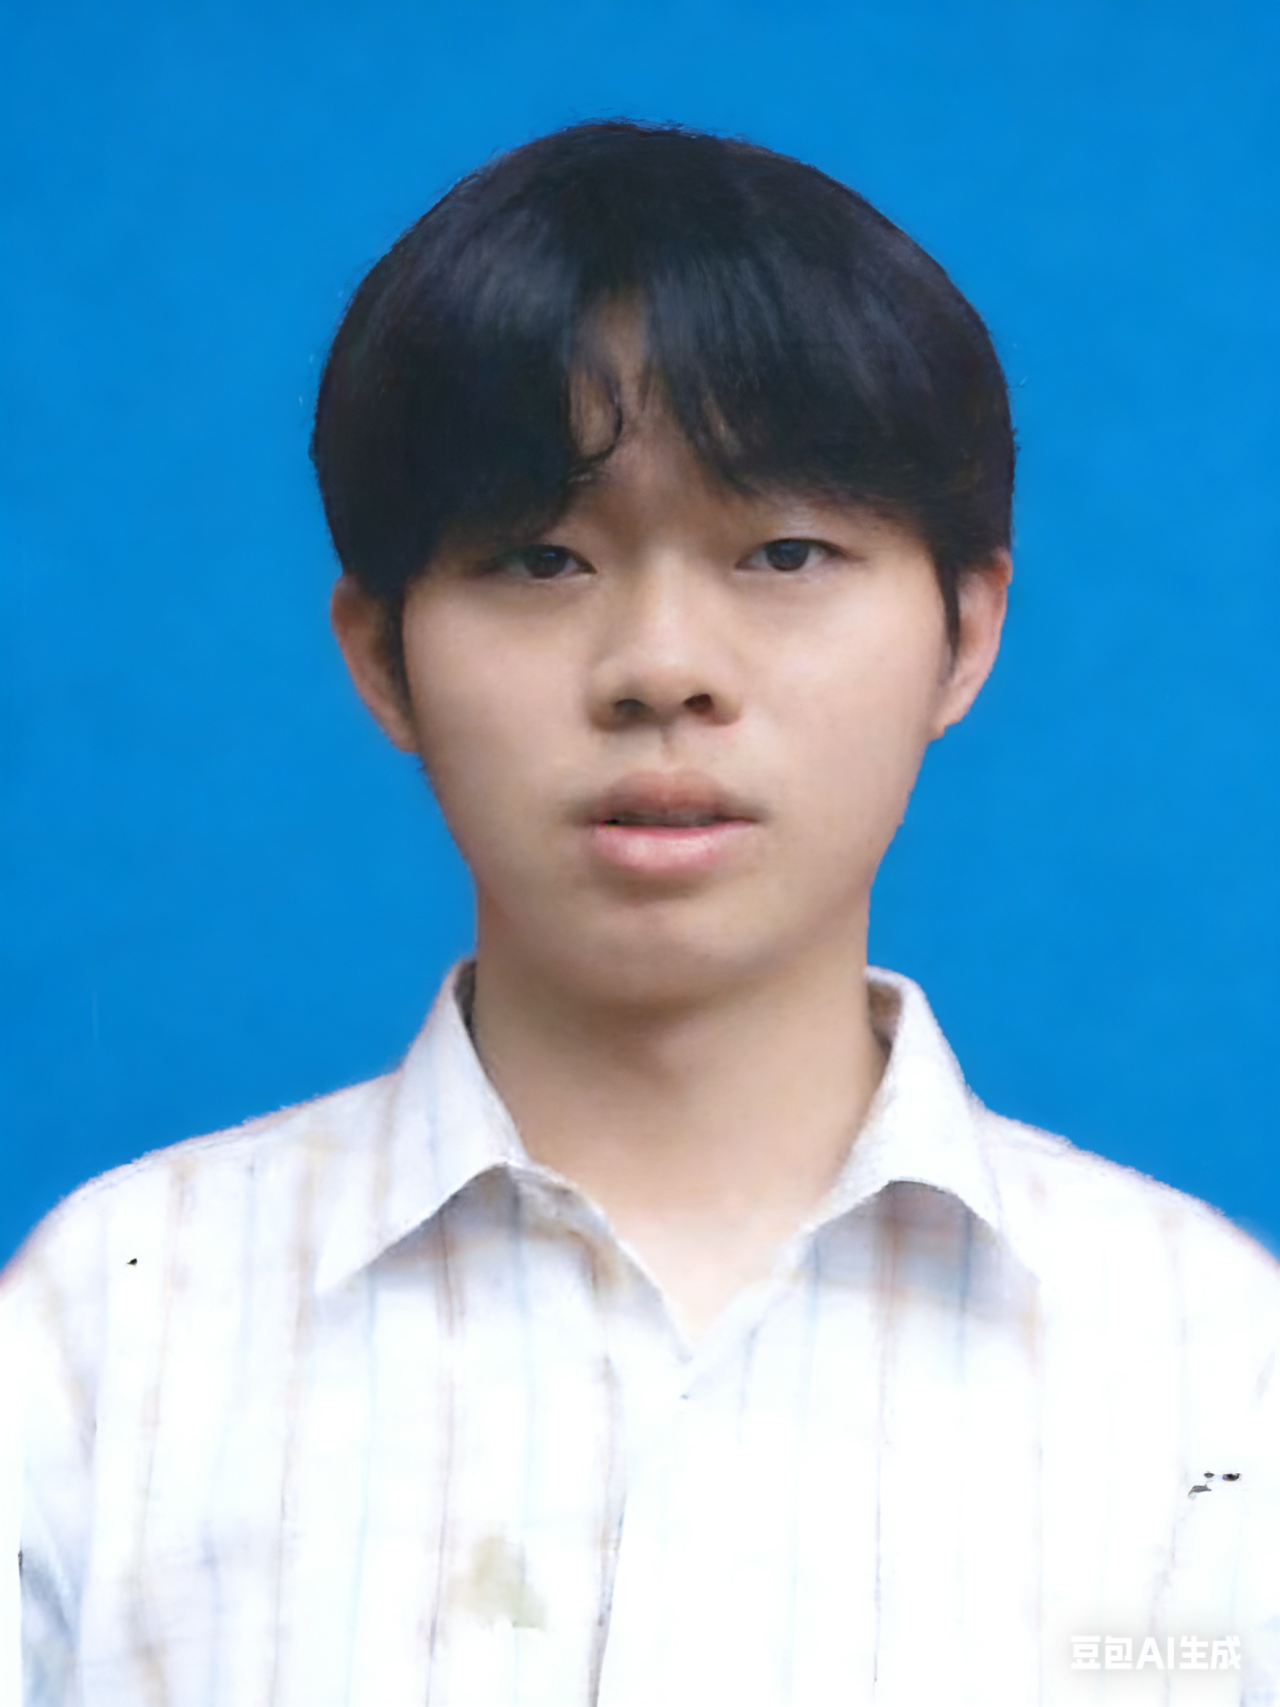
\includegraphics[height=4cm, width=3cm]{figures/teamMeambers/liTao.jpg} 
  \label{fig:liTao}
\end{wrapfigure}

\textbf{Tao Li} has a solid foundation in computer science and a strong spirit of exploration. 
He is proficient in Linux and Git, skilled in C and C++ programming, familiar with MPI and OpenMP parallel programming, and has a certain foundation in AI. 
In this competition, he mainly took charge of the design and analysis of the HPC system, and participated in the analysis and design of UnifoLM-WMA-0.

\vspace{4em}



% % 我们的参赛队伍由五名正式成员和多名后备成员组成，指导老师为林培英。参赛学生包括计算机科学与技术和网络空间安全专业的本科生，他们分别是沈华宇、裴杨坤、江龙、李涛(计算机科学与技术专业，大三)和陈牧远(网络空间安全专业，大二)。以下是每位队员的详细介绍。



% % 沈华宇，队长。他具备卓越的面对困难的能力、扎实的计算机科学功底以及勇于挑战的探索精神。熟练掌握 Linux 系统和 Git 版本控制工具，熟练掌握MPI 和 OpenMP 多线程编程以。曾在“蓝桥杯” Java 组获得省奖，参与开发过一个较为完善的在线学习平台以及基于遗传算法以及多模态优化的智能排课系统。在此次 ASC 竞赛中，作为队长，他不仅负责整体进度管理，还参与 AMSS-NCKU 的性能优化，通过并行计算以及内存管理提高了算法效率和速度。




% % 裴杨坤，掌握C/C++、Python 及 Shell 脚本跨平台开发，熟悉MPI、OpenMP 与 CUDA GPU 加速技术，具备多层级并行化算法设计与调优能力；熟悉 Linux 开发环境、CMake 编译工具链及 GCC/Intel 编译器高级优化选项。在本次比赛中，他负责AMSS-NCKU的部署运行及其优化方案的设计与实现。此外，他还完成了HPCG在CPU中的性能优化分析。



% %江龙，熟练掌握 C，C++，Java 和 pyhton 高级编程语言，拥有较强的算法设计与分析能力，能够快速适应不同的编程环境。深入掌握 MPI 和 OpenMP 并行编程模型，对 CUDA C 编程模型有着初步的理解，具有大规模并行计算和多线程编程的能力。熟悉 Linux 操作系统，熟练使用各类 Linux 命令，以 wsl2 作为日常开发平台，能够进行有效的模型部署和准确的测试结果。对传统算法具有较为扎实的基础，熟悉机器学习算法思想，具备人工智能（AI）基础。在本次比赛中主要负责 Embodied World Model Optimization部分，尝试采用 IO 优化、DeepCache 利用时序冗余的面训练策略，FlashAttention-2 优化和内核融合等方式加快 unifolm-wma 在 inference 时的速度。


% % 李涛，计算机基础扎实，富有探索精神。他熟练掌握Linux和Git，精通C和C++编程，并熟悉MPI和OpenMP并行编程，且具备一定人工智能（AI）基础。在此次比赛中，他主要负责HPC系统的设计与分析，并参与UnifoLM-WMA-0的分析与设计。

% % 陈牧远，热爱计算机，学习能力强。他熟练使用Linux和Git，精通C/C++和Java编程语言，具备强大的算法设计与实现能力，能够迅速适应不同的编程环境。熟悉模型推理安全，安全防护等技术。在这次比赛中，他主要负责HPCG GPU 优化部分和UnifoLM-WMA-0优化方案分析与设计。


\subsection{Team slogan}
\ 

\textbf{Code Flows, Nodes Ignite, Victory Follows.}

\clearpage
% \textbf{Unlimited Algorithms, Fearless Supercomputing, Victory Walks with Us}